\documentclass[11pt]{article}

\usepackage[margin=1in]{geometry}
\usepackage[T1]{fontenc}
\usepackage{lmodern}
\usepackage{microtype}
\usepackage{amsmath,amssymb,mathtools}
\usepackage{booktabs,tabularx,array}
\usepackage{enumitem}
\usepackage{xcolor}
\usepackage{graphicx}
\usepackage{tikz}
\usetikzlibrary{arrows.meta,positioning,fit}
\usepackage[round,authoryear]{natbib}
\usepackage[hidelinks]{hyperref}
\usepackage[nameinlink,noabbrev]{cleveref}

\definecolor{interaction}{HTML}{246BCE}
\definecolor{reasoning}{HTML}{7A3E9D}
\definecolor{audio}{HTML}{0B7A75}
\definecolor{ledger}{HTML}{9A6700}

\newcommand{\system}{\textsc{geno-voice}}
\newcommand{\vect}[1]{\boldsymbol{#1}}
\newcommand{\code}[1]{\texttt{#1}}
\newcolumntype{P}[1]{>{\raggedright\arraybackslash}p{#1}}
\newcolumntype{Y}{>{\raggedright\arraybackslash}X}
\setlength{\emergencystretch}{1.5em}

\title{Engineering Full-Duplex Voice Agents Around External Reasoning Models:\\
A Systems Survey and Reference Architecture}
\author{\system{} Project\\Technical Report}
\date{27 August 2026}

\begin{document}
\maketitle

\begin{abstract}
Full-duplex voice agents listen while speaking, handle overlap, and negotiate
the conversational floor without forcing rigid turns. Recent surveys organize
full-duplex spoken language models by synchronization strategy, model depth,
interaction ontology, and learned representation. This report addresses a
different engineering question: how can a duplex interaction layer retain an
external, configurable reasoning and tool-using model as the agent brain? We
synthesize 27 archived papers and three additional foundational/platform
sources into a modular reference architecture. The architecture separates acoustic cleanup,
target-speaker evidence, turn projection, interaction arbitration, asynchronous
reasoning, speech rendering, and two consistency ledgers. We argue for a
two-stage interruption protocol---reversible ducking followed by semantic
commit---and for a hard side-effect boundary around speculative inference. We
also propose an evaluation matrix that reports timing, arbitration, acoustic
robustness, context consistency, and tool correctness separately. The result is
a staged path from a cascaded local voice system to robust duplex behavior
without replacing its configured language-model endpoint.
\end{abstract}

\section{Introduction}

Human conversation is not a sequence of perfectly separated recordings.
Speakers pause, overlap, acknowledge, self-correct, and occasionally interrupt
one another. Cross-linguistic evidence also shows that turn exchange is rapid
but variable rather than governed by a fixed silence threshold
\citep{stivers2009turntaking}. A voice agent therefore needs more than voice
activity detection (VAD): it must infer the role and intent of an acoustic
event while its own speech is present.

Native full-duplex spoken language models such as Moshi, SyncLLM, SALM-Duplex,
F-Actor, DuplexSLA, DuplexOmni, and JoyAI-Talker learn some or all of this
behavior inside synchronized speech models
\citep{defossez2024moshi,veluri2024syncllm,hu2025salm,zufle2026factor,zhang2026duplexsla,huang2026duplexomni,bai2026joytalker}.
This line establishes an important behavioral ceiling, but it is not always a
product fit. Coding and tool-using agents often need to preserve a configured
reasoning endpoint, enterprise routing, model governance, and a mature action
loop. Replacing that brain with a speech foundation model changes the product
rather than merely adding voice.

This report surveys the complementary systems path: a real-time interaction
layer around an external reasoning model. Its contributions are:

\begin{enumerate}[leftmargin=*]
  \item a signal-to-action decomposition connecting AEC, personalized speech
        evidence, semantic endpointing, duplex arbitration, tools, and TTS;
  \item a reversible interruption protocol that separates audible responsiveness
        from irreversible conversational and tool state;
  \item explicit heard-prefix and committed-action ledgers for consistency; and
  \item a component-level evaluation program grounded in recent duplex
        benchmarks.
\end{enumerate}

\section{Scope and Relationship to Existing Surveys}

The broad WavChat survey organizes spoken dialogue systems, representations,
training, streaming, and evaluation across both cascaded and end-to-end models
\citep{ji2024wavchat}. Two dedicated full-duplex surveys then sharpen the
space. \citet{chen2025fdsurvey} distinguish engineered from learned
synchronization and group evaluation into temporal, behavioral, semantic, and
acoustic pillars. \citet{lu2026fdsurvey} introduce an L0--L3 architecture
hierarchy, a $T\times I\times R$ interaction ontology, and an
\code{IDLE/LISTEN/SPEAK/WAIT/DUAL} state machine.

\Cref{tab:surveys} shows why another general taxonomy would be redundant. Our
scope is instead the deployment boundary between a duplex voice layer and an
external reasoning/tool agent. We include native models as behavioral
references, but focus on components that can be measured, replaced, and
integrated independently.

\begin{table}[ht]
\centering
\caption{Relationship to prior surveys. ``External brain'' means a separately
configured language-model and tool runtime rather than the speech model's own
reasoner.}
\label{tab:surveys}
\begin{tabularx}{\textwidth}{@{}P{0.20\textwidth}P{0.25\textwidth}Y@{}}
\toprule
Work & Primary organizing idea & Main distinction from this report \\
\midrule
WavChat \citep{ji2024wavchat} & Cascaded vs. end-to-end spoken dialogue & Broader model, representation, and training survey \\
Chen and Yu \citep{chen2025fdsurvey} & Engineered vs. learned synchronization & Full-duplex model taxonomy and four-pillar evaluation \\
Lu et al. \citep{lu2026fdsurvey} & L0--L3 hierarchy, $T\times I\times R$, five-state machine & Architectural and interaction ontology across claimed duplex systems \\
This report & Replaceable interaction layer around an external brain & AEC, target-speaker gating, reversible interruption, ledgers, safe tools, and deployment order \\
\bottomrule
\end{tabularx}
\end{table}

\section{Operational Definition and Signal Model}

We use \emph{full duplex} for a system that continuously accepts user audio
while rendering assistant audio and can make interaction decisions from their
overlap. This definition describes an interface capability, not proof that the
system behaves well. A push-to-talk system is half duplex; a system that merely
stops TTS whenever VAD fires is interruptible but behaviorally fragile; a
capable duplex system distinguishes at least echo, noise, backchannel,
other-addressed speech, hesitation, and substantive interruption.

Let $u_t$ be near-end target-user speech, $r_t$ the exact assistant render
signal, $h_t$ the room/device echo path, and $v_t$ all other interference. The
microphone observes

\begin{equation}
  m_t = u_t + (h_t * r_t) + v_t,
  \label{eq:mixture}
\end{equation}

where $*$ denotes convolution. The front end estimates the echo path and
produces

\begin{equation}
  e_t = m_t - (\hat h_t * r_t) \approx u_t + v_t.
  \label{eq:aec}
\end{equation}

This is why acoustic echo cancellation (AEC) belongs inside the system
boundary. Apple voice processing and WebRTC AudioProcessing both use the
render path as a reference rather than asking a language model to infer its own
playback from a contaminated transcript
\citep{apple2026voiceprocessing,webrtc2026apm}.

The interaction layer observes a feature vector

\begin{equation}
\vect z_t = [p_{\mathrm{speech}}, p_{\mathrm{target}},
\rho_{\mathrm{echo}}, \vect h^{\mathrm{audio}}_t,
\vect h^{\mathrm{text}}_t, q_t, \ell_t],
\label{eq:evidence}
\end{equation}

where $q_t$ is dialogue state and $\ell_t$ is playback-ledger state. VAD is one
feature, not the policy.

\section{Architecture Families}

\subsection{Native synchronized speech models}

dGSLM demonstrates that two streams of discrete speech units can learn
turn-taking and overlap jointly without a text bottleneck
\citep{nguyen2022dgslm}. Voice Activity Projection (VAP) provides a related
discriminative view by predicting both speakers' future activity rather than
only current voice presence \citep{ekstedt2022vap}; later work demonstrates
real-time operation and backchannel prediction
\citep{inoue2024realtimevap,inoue2024backchannel}.

Modern native systems place synchronized user and assistant streams on a
shared clock. SyncLLM time-aligns fixed audio chunks
\citep{veluri2024syncllm}; Moshi combines user audio, assistant audio, and an
assistant inner-monologue text stream \citep{defossez2024moshi}; SALM-Duplex
fuses a streaming speech encoder with text and codec outputs
\citep{hu2025salm}. These designs reduce hand-built boundaries but couple
dialogue policy, language reasoning, and speech generation.

F-Actor adds instruction control over voice and conversational behavior
\citep{zufle2026factor}; DuplexSLA adds a synchronized action channel
\citep{zhang2026duplexsla}; JoyAI-Talker separates a Thinker, expressive
Talker, and plug-in duplex gate \citep{bai2026joytalker}. These advances inform
interfaces even when their full models are not adopted.

\subsection{Pluggable interaction controllers}

FlexDuo wraps a half-duplex dialogue system with an audio window, context
manager, state manager, and seven-action controller
\citep{liao2025flexduo}. A smaller semantic dialogue manager predicts four
listen/speak control tokens after AEC, VAD, and ASR
\citep{zhang2025manager}. FireRedChat is the closest released production-shaped
reference: personalized VAD (pVAD) rejects non-primary speakers, semantic
end-of-turn detection decides completion, and a replaceable dialogue manager
handles tools and context \citep{chen2025firered}.

DuplexOmni generalizes this seam into a fast interaction layer and an
asynchronous thinking layer \citep{huang2026duplexomni}. That split is the
best match for an external reasoning endpoint: interaction never waits for deep
reasoning, and obsolete thinking can be superseded when the user changes the
task.

\section{Reference Architecture}

\Cref{fig:architecture} synthesizes the literature into a modular path. The
front end removes known playback and estimates target-speaker evidence. A fast
acoustic path reacts immediately; a streaming semantic path gathers partial
text and prosody. The arbiter emits typed decisions. The external agent and TTS
operate asynchronously, while ledgers retain what was heard and what actions
were committed.

\begin{figure}[ht]
\centering
\resizebox{0.97\textwidth}{!}{%
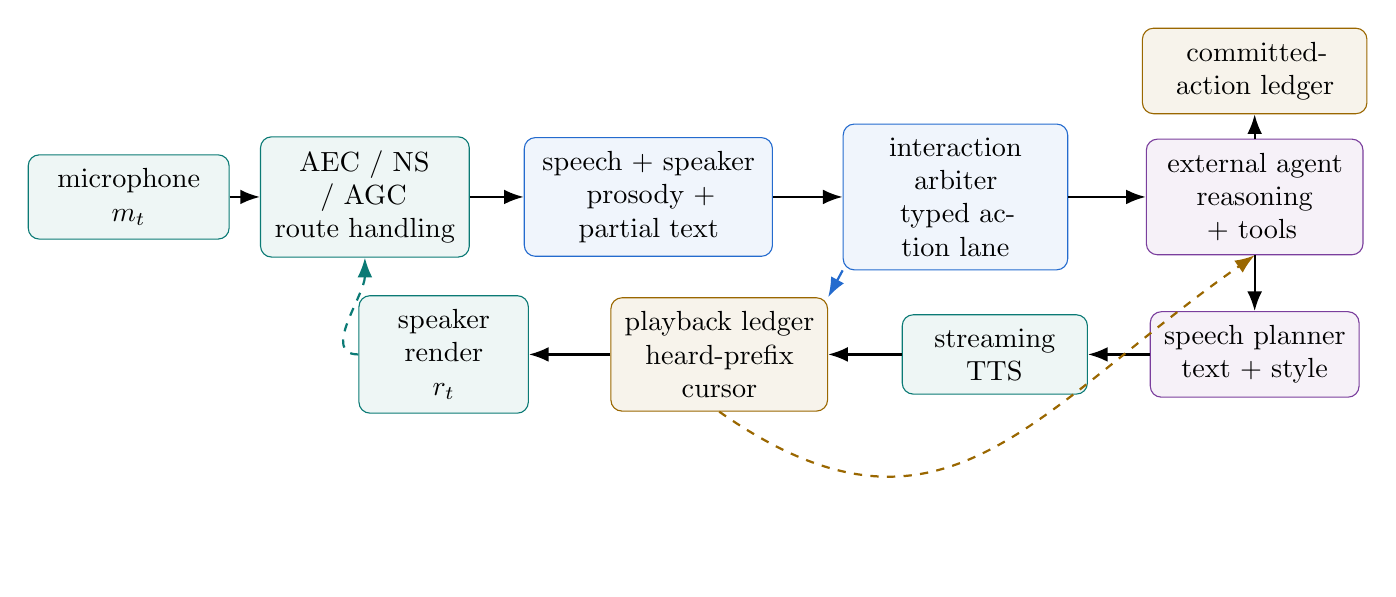
\begin{tikzpicture}[
  box/.style={draw, rounded corners, minimum height=10mm, align=center, inner sep=5pt},
  audioBox/.style={box, draw=audio, fill=audio!7},
  interactionBox/.style={box, draw=interaction, fill=interaction!7},
  reasoningBox/.style={box, draw=reasoning, fill=reasoning!7},
  ledgerBox/.style={box, draw=ledger, fill=ledger!8},
  flow/.style={-{Latex[length=2.5mm]}, thick}
]
  \node[audioBox, text width=22mm] (mic) at (0,0) {microphone\\$m_t$};
  \node[audioBox, text width=23mm] (front) at (3.0,0) {AEC / NS / AGC\\route handling};
  \node[interactionBox, text width=28mm] (features) at (6.6,0) {speech + speaker\\prosody + partial text};
  \node[interactionBox, text width=25mm] (arbiter) at (10.5,0) {interaction arbiter\\typed action lane};
  \node[reasoningBox, text width=24mm] (brain) at (14.3,0) {external agent\\reasoning + tools};
  \node[reasoningBox, text width=23mm] (planner) at (14.3,-2.0) {speech planner\\text + style};
  \node[audioBox, text width=20mm] (tts) at (11.0,-2.0) {streaming TTS};
  \node[ledgerBox, text width=24mm] (playback) at (7.5,-2.0) {playback ledger\\heard-prefix cursor};
  \node[audioBox, text width=18mm] (render) at (4.0,-2.0) {speaker render\\$r_t$};
  \node[ledgerBox, text width=25mm] (tools) at (14.3,1.6) {committed-action ledger};

  \draw[flow] (mic) -- (front);
  \draw[flow] (front) -- (features);
  \draw[flow] (features) -- (arbiter);
  \draw[flow] (arbiter) -- (brain);
  \draw[flow] (brain) -- (planner);
  \draw[flow] (planner) -- (tts);
  \draw[flow] (tts) -- (playback);
  \draw[flow] (playback) -- (render);
  \draw[flow] (brain) -- (tools);
  \draw[flow, audio, dashed]
    (render.west) to[out=180,in=-90] (front.south);
  \draw[flow, interaction]
    (arbiter.south west) -- (playback.north east);
  \draw[flow, ledger, dashed]
    (playback.south) to[out=-35,in=-145,looseness=1.25] (brain.south);
\end{tikzpicture}%
}
\caption{Reference architecture for a duplex voice layer around an external
reasoning and tool agent. Black arrows show the primary data flow; the blue
arrow controls playback; the dashed teal arrow supplies the exact render
reference; and the dashed ochre arrow reconciles the heard prefix.}
\label{fig:architecture}
\end{figure}

\subsection{Target-speaker and interference gating}

AEC answers whether audio resembles the assistant render. It does not answer
whether residual speech belongs to the intended user. FireRedChat addresses the
latter with pVAD \citep{chen2025firered}. IRAF learns a causal reliability gate
from a target-speaker embedding $\vect s$ and user-audio embedding $\vect x_t$
\citep{zhong2026iraf}:

\begin{equation}
  g_t = 2\,\sigma\!\left(f_\psi(\vect s,\vect x_{\le t})\right),
  \qquad \tilde{\vect x}_t=g_t\vect x_t.
  \label{eq:iraf}
\end{equation}

For a modular system, $p_{\mathrm{target}}$ should remain visible alongside
$p_{\mathrm{speech}}$ and echo residual. Collapsing them into one opaque score
makes route changes and double-talk failures difficult to diagnose.

\subsection{Turn projection and endpointing}

VAP estimates future joint voice activity; textual models estimate syntactic
and pragmatic completion. Their errors are complementary in conversational HRI
\citep{skantze2025hri}. FastTurn combines streaming CTC text, acoustic
representations, and a semantic model to distinguish complete, incomplete,
backchannel, and wait events \citep{wang2026fastturn}. SpeculativeETD uses a
cheap streaming detector and invokes a larger endpoint model only near a
possible boundary \citep{ok2025speculative}.

Binary endpoint labels discard useful duration information. Next-Turn predicts

\begin{equation}
  \tau_t = t_{\mathrm{next\ onset}}-t,
  \label{eq:nextturn}
\end{equation}

which can be trained from timestamps and fused with endpoint probability
\citep{tsoi2026nextturn}. Endpoint Anticipation instead forecasts completion
far enough ahead to prepare a short LLM/TTS continuation privately
\citep{udupa2026anticipation}. These are performance signals, not permission to
commit user intent.

\section{Interaction Arbitration and Reversible Interruption}

Let $Y_t$ be the latent event class (echo, noise, backchannel,
other-addressed speech, hesitation, or substantive interruption) and
$\mathcal A$ the controller actions. A calibrated policy minimizes asymmetric
risk:

\begin{equation}
  a_t^*=\arg\min_{a\in\mathcal A}
  \mathbb E\!\left[L(a,Y_t)\mid \vect z_{\le t}\right].
  \label{eq:risk}
\end{equation}

The loss should make audible talk-over expensive, but should also make
destructive false cancellation more expensive than a brief duck. This motivates
two phases:

\begin{enumerate}[leftmargin=*]
  \item \textbf{Reversible onset response.} Likely target speech immediately
        ducks or pauses playback. The agent request and remaining PCM stay
        resumable while 200--400 ms of evidence accumulates.
  \item \textbf{Semantic commit.} A substantive interruption cancels future
        playback, drains stale capture, supersedes obsolete reasoning, and
        commits the new user turn. Echo, noise, backchannel, and other-addressed
        speech resume from the playback cursor.
\end{enumerate}

This protocol makes reaction time depend on a fast acoustic path without giving
that path authority over irreversible state. Session policy should also be
configurable: F-Actor shows that backchannel and interruption behavior can be
instruction-controlled rather than globally fixed \citep{zufle2026factor}.

\section{External Reasoning, Tools, and Consistency}

The interaction layer needs a narrow contract with the external agent:

\begin{verbatim}
submit_committed_turn(transcript, timing, interruption_context)
supersede_response(response_id, heard_assistant_prefix)
receive_text_delta(response_id, text)
receive_tool_event(response_id, event)
\end{verbatim}

The contract is deliberately text-and-event based. A custom endpoint can be
replaced without teaching the acoustic controller about model vendors.

\subsection{Heard-prefix ledger}

If response text $T_r$ has been synthesized but playback cursor $k_r(t)$ has
only crossed a prefix, conversational history must contain

\begin{equation}
  H_r(t)=T_r[0:k_r(t)],
  \label{eq:heardprefix}
\end{equation}

not the generated-but-unheard suffix. Otherwise the reasoning model believes
the user heard facts or instructions that never reached the speaker. The
playback ledger associates response IDs, text spans, PCM chunks, render
timestamps, route changes, and cancellation state.

\subsection{Committed-action ledger}

Speech cancellation cannot undo a file edit or network side effect. Tool
events therefore need a separate append-only ledger with proposed, authorized,
started, committed, failed, and compensated states. DuplexSLA's distinct action
lane supports this separation \citep{zhang2026duplexsla}. A predicted endpoint
may initiate side-effect-free text/TTS speculation, but no mutating tool call
may cross the commit boundary before the user turn is confirmed.

\section{Speech Rendering and Expressivity}

Native speech models preserve prosody because audio remains inside the model;
cascaded systems often flatten intent into plain text. A modular compromise is
a speech-plan object

\begin{equation}
  p_i=(\text{text}_i,\text{intent}_i,\text{rate}_i,
       \text{pause}_i,\text{emphasis}_i,\text{affect}_i)
  \label{eq:speechplan}
\end{equation}

for every speakable clause. The external agent supplies semantics; a local
planner assigns delivery; TTS renders incrementally. JoyAI-Talker's expressive
Talker and F-Actor's promptable conversational behavior provide model-scale
evidence for this interface \citep{bai2026joytalker,zufle2026factor}. Duplex
correctness must not depend on any one TTS engine.

\section{Evaluation}

No scalar ``duplex score'' is sufficient. A system can appear highly responsive
by cancelling on every noise burst. Evaluation should report the five groups in
\Cref{tab:metrics} separately.

\begin{table}[ht]
\centering
\caption{Component-level evaluation for modular duplex agents.}
\label{tab:metrics}
\begin{tabularx}{\textwidth}{@{}P{0.18\textwidth}Y Y@{}}
\toprule
Group & Example metrics & Failure exposed \\
\midrule
Acoustic & echo return loss enhancement, residual echo, double-talk recall, target-speaker confusion & self-barge and non-target activation \\
Timing & endpoint latency, stop latency, resume gap, audible response latency & sluggishness or premature response \\
Arbitration & interruption recall, false abandon, backchannel/background false stop & wrong conversational action \\
Consistency & heard-prefix accuracy, stale-frame count, superseded-response leakage & mismatch between heard and modeled history \\
Tools & argument accuracy, stale action rate, unauthorized speculative effects, compensation rate & real-world side effects from unstable turns \\
\bottomrule
\end{tabularx}
\end{table}

For AEC, a useful diagnostic is echo return loss enhancement

\begin{equation}
  \operatorname{ERLE}=10\log_{10}
  \frac{\mathbb E[d_t^2]}{\mathbb E[e_t^2]},
  \label{eq:erle}
\end{equation}

where $d_t$ is microphone echo before cancellation and $e_t$ residual echo.
ERLE must be paired with double-talk tests: suppressing both echo and the real
user is not success.

Full-Duplex-Bench v1.5 isolates respond-versus-resume behavior under overlap
\citep{lin2025fdb15}; v2 adds automated multi-turn examination
\citep{lin2025fdb2}; v3 combines real disfluency with chained tool use
\citep{lin2026fdb3}. HumDial-FDBench contributes real dual-channel human
conversations and a public challenge framework \citep{wang2026humdial}. These
external benchmarks should complement deterministic virtual-microphone tests
with configurable room delay, gain, filtering, jitter, and overlap.

\section{Implementation Roadmap}

The literature supports the following order for a local modular system:

\begin{enumerate}[leftmargin=*]
  \item \textbf{Audio front end.} Add macOS voice processing with an exact
        render reference; retain WebRTC AudioProcessing as the cross-platform
        candidate. Log pre/post AEC, route changes, and underruns.
  \item \textbf{Reversible playback.} Replace immediate energy-triggered
        cancellation with duck, classify, then resume or commit.
  \item \textbf{Endpoint model.} Combine a small audio-native end-of-turn model
        with partial-text completion while preserving the silence fallback.
  \item \textbf{Five-class arbiter.} Begin with calibrated rules for
        \code{HOLD\_USER}, \code{TAKE\_TURN}, \code{CONTINUE\_AGENT},
        \code{YIELD\_AGENT}, and \code{IGNORE\_INPUT}; train only after labeled
        feature traces exist.
  \item \textbf{Ledgers and agent bridge.} Reconcile the heard prefix and
        committed tool effects on interruption and supersession.
  \item \textbf{Safe anticipation.} Cache short speculative text/TTS output
        only after correctness is established; never speculatively mutate.
  \item \textbf{Expressivity and native baselines.} Add speech planning, then
        compare against obtainable native systems without changing the external
        brain contract.
\end{enumerate}

\section{Open Problems}

\paragraph{Robust target identity.}
Speaker embeddings drift across microphones, distance, illness, and noise.
The field lacks a broadly validated target-speaker gate under simultaneous
assistant render and near-end speech.

\paragraph{Training labels for intent under overlap.}
Public corpora contain far less annotated echo, other-addressed speech,
backchannel, self-correction, and tool-state revision than clean turns. The
recent surveys identify this realization gap
\citep{chen2025fdsurvey,lu2026fdsurvey}.

\paragraph{Latency versus semantic authority.}
Endpoint anticipation can hide sequential delay, but premature semantic or tool
commit is costly. Better calibrated uncertainty and explicit rollback domains
are needed.

\paragraph{Cross-platform acoustic control.}
OS voice-processing graphs and WebRTC APM have different routing, device, and
latency behavior. Reproducible duplex evaluation must include real devices, not
only clean WAV files.

\paragraph{Expressivity without policy coupling.}
Native models jointly learn wording, timing, and voice. Modular systems need
interfaces that preserve paralinguistic intent while keeping the agent,
controller, and renderer independently replaceable.

\section{Conclusion}

The duplex literature does not imply that every voice product should train a
native speech foundation model. It does imply that turn-taking is a continuous,
multi-signal control problem. For agents whose value lies in an existing
reasoning and tool loop, the strongest design is a deep interaction module:
clean the signal with an exact render reference, retain target-speaker and
semantic evidence separately, react reversibly, commit deliberately, and
record both heard speech and irreversible actions. This architecture captures
the interaction/thinking split emerging in recent models while preserving the
configured external brain.

\bibliographystyle{unsrtnat}
\bibliography{references}

\end{document}
